% !TEX program = pdflatex
%%%%%%%%%%%%%%%%%%%%%%%%%%%%%%%%%%%%%%%%%%%%%%%%%%%%%%%%%%%%%%%%%%%%%%%%%%%%%%%%
% GTM Agent — Final Report (all four deliverables combined into one PDF)
% Course: Foundations and Application of Generative AI
%
% Build:
%   pdflatex FinalReport.tex   (run twice for the table of contents)
%%%%%%%%%%%%%%%%%%%%%%%%%%%%%%%%%%%%%%%%%%%%%%%%%%%%%%%%%%%%%%%%%%%%%%%%%%%%%%%%

% \documentclass is declared HERE (not in Praeambel) so the editor detects
% THIS file as the compile root. The rest of the preamble is loaded below.
\documentclass[fontsize=11pt,twoside=off]{scrbook}
%%%%%%%%%%%%%%%%%%%%%%%%%%%%%%%%%%%%%%%%%%%%%%%%%%%%%%%%%%%%%%%%%%%%%%%%%%%%%%%%
% Preamble — based on the official TUM "Wissenschaftliche Arbeit" template,
% adapted for the GTM Agent combined final report (4 parts in one PDF).
% NOTE: biblatex/biber is intentionally NOT used here (no biber binary in this
% build environment); references are typeset as a plain list per chapter instead.
%%%%%%%%%%%%%%%%%%%%%%%%%%%%%%%%%%%%%%%%%%%%%%%%%%%%%%%%%%%%%%%%%%%%%%%%%%%%%%%%

% NOTE: \documentclass is declared in FinalReport.tex (the main file), not here,
% so the editor detects FinalReport.tex as the compile root. This file is loaded
% right after \documentclass, so it may start issuing \usepackage immediately.
\usepackage{scrlayer-scrpage} % customizable headers/footers

\usepackage[utf8]{inputenc} % text encoding: UTF-8
\usepackage[T1]{fontenc}    % font encoding

\usepackage[english]{babel} % English localization
\usepackage{graphicx}       % graphics
\usepackage{float}          % [H] placement: pin figures/tables exactly in place
\usepackage{tikz}           % simple flow diagram in the User Guide
\usetikzlibrary{positioning,arrows.meta}
\tikzset{flowbox/.style={draw, rounded corners, fill=black!4, align=center,
  font=\footnotesize, minimum height=9mm, text width=18mm, inner sep=2pt}}
\usepackage{amsmath}        % math
\usepackage{booktabs}       % nicer table rules (\toprule, \midrule, \bottomrule)
\usepackage{longtable}      % tables that span pages
\usepackage{xltabular}      % longtable + tabularx X column (cross-page balanced tables)
\usepackage{array}
\usepackage{etoolbox}       % \ifdefempty etc. (used by the title page)

% Font Helvetica (TUM corporate design):
\usepackage[scaled]{helvet}
\renewcommand{\familydefault}{\sfdefault}

% Hyphenation:
\usepackage{hyphenat}
\hyphenation{TUM Figure Figures GTM}

\usepackage[hidelinks]{hyperref}          % hyperlinks
\usepackage[onehalfspacing]{setspace}     % 1.5 line spacing
\usepackage{calc}      % length calculations
\usepackage{enumitem}  % more control over list environments
\usepackage{relsize}   % relative font sizing
\usepackage{tabularx}  % flexible tables
\usepackage[tablewithout, figurewithout]{caption} % caption customization

% Continuous numbering of figures & tables (instead of per-chapter):
\usepackage{chngcntr}
\counterwithout{figure}{chapter}
\counterwithout{table}{chapter}

% Special command definitions:
\newcommand{\Thema}{}

\usepackage{bookmark} % PDF bookmarks

% A few Unicode characters used in the source Markdown are not in pdfLaTeX's
% default inputenc table; map them explicitly.
\usepackage{newunicodechar}
\newunicodechar{§}{\S}
\newunicodechar{·}{\textperiodcentered}
\newunicodechar{→}{\ensuremath{\rightarrow}}
\newunicodechar{↔}{\ensuremath{\leftrightarrow}}
\newunicodechar{≤}{\ensuremath{\leq}}
\newunicodechar{≥}{\ensuremath{\geq}}

% Emoji -> monochrome icons. pdfLaTeX has no emoji font, so 👍 / 👎 would error;
% these map them to FontAwesome thumbs, letting the source keep using the emoji.
\usepackage{fontawesome5}
\newunicodechar{👍}{\faThumbsUp}
\newunicodechar{👎}{\faThumbsDown}

% Helper macro emitted by pandoc for compact lists:
\providecommand{\tightlist}{%
  \setlength{\itemsep}{0pt}\setlength{\parskip}{0pt}}

% All report images are read directly from the repo's Reports/Screenshots/ folder
% (single source of truth — no duplicate copy). The path is RELATIVE to
% FinalReport.tex: FinalReport -> Reports_output -> mei_doc -> repo root, then
% Reports/Screenshots/. If you move the FinalReport folder, update this line.
% With this, \includegraphics{Foo.png} and \screenshot{Foo.png} find the file by
% its bare name, so use the real filenames from Reports/Screenshots (spaces are
% not allowed by graphicx, but parentheses are fine).
\graphicspath{{../../../Reports/Screenshots/}}

% Screenshot helper: \screenshot[short caption]{file}{caption}. Keeps figures
% readable and consistent across the User Guide. The optional first argument is
% the short form used in the List of Figures; it defaults to the full caption.
\newcommand{\screenshot}[3][\relax]{%
  \begin{figure}[htbp]
    \centering
    \includegraphics[width=0.95\linewidth]{#2}%
    \ifx\relax#1\relax\caption{#3}\else\caption[#1]{#3}\fi
  \end{figure}%
}

% Reference-list entry: APA-style hanging indent.
\newcommand{\refitem}[1]{\par\noindent\hangindent=8mm\hangafter=1 #1\par\vspace{1.4mm}}

% Suppress layout-related warnings:
\usepackage[immediate]{silence}
\WarningFilter[layout]{latex}{Reference `LastPage'}
\WarningFilter[layout]{lastpage}{Rerun to get the references right}
\WarningFilter[layout]{latex}{Label(s) may have changed.}
\WarningFilter[layout]{textpos}{environment textblock* not in vertical mode}
\WarningFilter[layout]{scrbook}{Change of }
\WarningFilter[layout]{tocbasic}{number width of}
\WarningFilter{latex}{Font shape declaration has incorrect series value} % harmless psnfss t1phv.fd quirk

% Debugging:
%\DeactivateWarningFilters[layout]
%\usepackage{showframe}


%=============================================================================
%  >>> REPORT METADATA <<<
%=============================================================================
\newcommand{\ReportTitle}{GTM Agent}
\newcommand{\ReportSubtitle}{}
\newcommand{\Course}{Foundations and Application of Generative AI}
\newcommand{\Term}{Summer Semester 2026}
\newcommand{\Lecturer}{Prof.\ Dr.\ Chunyang Chen}
\newcommand{\Chair}{Chair of Software Engineering \& AI}
\newcommand{\School}{TUM School of Computation, Information and Technology}
\newcommand{\GroupName}{Group2}
\newcommand{\TeamMembers}{%
    Jingyi Shao      & 03798142 \\
    Sihao Tao        & 03793452 \\
    Swaraj Shrestha  & 03816043 \\
    Trinh Nguyen     & 03824365 \\
    Xinyi Li         & 03814492 \\
    Yilang Mei       & 03759865 \\
    Zijian Luo       & 03817807%
}
\newcommand{\SubmissionDate}{\today}

%%%%%%%%%%%%%%%%%%%%%%%%%%%%%%%%%%%%%%%%%%%%%%%%%%%%%%%%%%%%%%%%%%%%%%%%%%%%%%%%
% EINSTELLUNGEN
%%%%%%%%%%%%%%%%%%%%%%%%%%%%%%%%%%%%%%%%%%%%%%%%%%%%%%%%%%%%%%%%%%%%%%%%%%%%%%%%

\KOMAoptions{parskip=full}


% Seitenränder:
% NOTE: left/right symmetrised to 25mm for PDF submission (the original TUM
% thesis template used 40mm inner / 21mm outer as a physical binding margin,
% which is unnecessarily wide on the left for a screen-read report).

\newcommand{\SeitenrandOben}{25.8mm}
\newcommand{\SeitenrandRechts}{25mm}
\newcommand{\SeitenrandLinks}{25mm}
\newcommand{\SeitenrandUnten}{24.8mm}
\newcommand{\FusszeileHoehe}{11.7mm}

\usepackage[a4paper,
    head=\SeitenrandOben,
    top=\SeitenrandOben,
    bottom=\SeitenrandUnten,
    inner=\SeitenrandLinks,
    outer=\SeitenrandRechts
]{geometry}


% Fußzeilen:

\setlength{\footheight}{\FusszeileHoehe}
\clearscrheadfoot
% Footer: report title (left, width-limited so a long title cannot collide with
% the group/page), group number and page number (right).
\ifoot*{\parbox[b]{.66\textwidth}{\raggedright\ReportTitle}\vfill}
\ofoot*{\GroupName\quad\textbar\quad\pagemark\vfill}
\setkomafont{pageheadfoot}{\fontsize{9pt}{13pt}\normalfont}
\setkomafont{pagefoot}{\bfseries}
\setkomafont{pagenumber}{\normalfont}
\pagestyle{scrheadings}


% Fußnoten:

\KOMAoptions{%
    footnotes=multiple % mehrere Fußnoten werden durch Zeichen getrennt
}
%\setfootnoterule[.6pt]{5.08cm}
\renewcommand{\footnoterule}{\hrule width 5.08cm height .6pt \vspace*{3.9mm}}
%\setlength{\footnotesep}{5mm}
\deffootnote{2mm}{2mm}{%
    \makebox[2mm][l]{\textsuperscript{\thefootnotemark}}%
}
\setkomafont{footnoterule}{\fontsize{9pt}{20pt}\selectfont}


% Überschriften:

\KOMAoptions{%
    open=any, % keine Festlegung auf linke oder rechte Seite
    numbers=noendperiod, % kein automatischer Punkt nach Gliederungsnummer
    headings=small
}

\makeatletter
\g@addto@macro{\@afterheading}{\vspace{-\parskip}} % \parskip nach Gliederungsbefehlen entfernen
\renewcommand*{\chapterheadstartvskip}{\vspace{\@tempskipa}\vspace{-3pt}} % Korrektur für Abstand über Kapitelüberschriften
\makeatother

\setkomafont{disposition}{\normalfont\sffamily}

\setkomafont{chapter}{\normalfont\bfseries\fontsize{19pt}{22pt}\selectfont}
\RedeclareSectionCommand[%
  beforeskip=0pt,
  afterskip=29pt,
]{chapter}
\renewcommand*{\chapterformat}{\thechapter.\enskip} % Immer Punkt nach Kapitelnummer

\setkomafont{section}{\bfseries\fontsize{15pt}{17pt}\selectfont}
\RedeclareSectionCommand[%
  beforeskip=0pt,
  afterskip=24.1pt
]{section}
\renewcommand*{\sectionformat}{\makebox[13mm][l]{\thesection.\enskip}} % Feste Breite für Abschnittsnummer und immer Punkt danach

\setkomafont{subsection}{\bfseries\fontsize{12pt}{13pt}\selectfont}
\RedeclareSectionCommand[%
  beforeskip=0pt,
  afterskip=1pt
]{subsection}
\renewcommand*{\subsectionformat}{\makebox[13mm][l]{\thesubsection.\enskip}} % Feste Breite für Unterabschnittsnummer und immer Punkt danach


% Listen:

\setlist{%
    labelsep=0mm,
    itemindent=0pt,
    labelindent=0pt,
    align=left,
    parsep=1.5ex
}
\setlist[itemize]{%
    leftmargin=5mm,
    labelwidth=4.9mm
}
\setlist[itemize,1]{%
    before={\vspace{0.25ex}},
    label={\raisebox{.35ex}{\smaller[2]\textbullet}},
    after={\vspace{-\parsep}\vspace{-.25ex}}
}
\setlist[itemize,2]{%
    label={\raisebox{.35ex}{\rule{.58ex}{.58ex}}}
}
\setlist[enumerate]{%
    leftmargin=10mm,
    labelwidth=9.9mm
}
\setlist[enumerate,2]{%
    label={\alph*.}
}

\setlist[description]{%
%    labelindent=!,
    leftmargin=1em,
    labelwidth=!,
    parsep=0mm,
    partopsep=0mm,
    labelsep=1em,
}


% Verzeichnisse:

\KOMAoptions{%
    toc=graduated, % hierarchische Einrückung (1.1/1.2 unter 1 eingerückt)
    toc=chapterentrydotfill, % Punkte bis zur Seitennummer bei Kapiteln
    listof=entryprefix, % Präfix für Einträge in Abbildungs- und Tabellenverzeichnis
    listof=nochaptergap, % Kein Abstand für Kapiteleinträge in extra Verzeichnissen
}

\makeatletter
\renewcommand{\@dotsep}{.3} % Abstand der Füllpunkte

% "chapteratlist" für Inhaltsverzeichnis auswerten:
\renewcommand*{\addchaptertocentry}[2]{%
  %\Iftocfeature{toc}{chapteratlist}{}{%
    \addtocontents{toc}{\protect\vspace{-10pt}}% extra Abstand vor Kapitelüberschriften in Inhaltsverzeichnis entfernen
  %}%
  % Originaldefinition aus scrbook.cls:
  \addtocentrydefault{chapter}{#1}{#2}%
  \if@chaptertolists
    \doforeachtocfile{%
      \Iftocfeature{\@currext}{chapteratlist}{%
        \addxcontentsline{\@currext}{chapteratlist}[{#1}]{#2}%
      }{}%
    }%
    \@ifundefined{float@addtolists}{}{\scr@float@addtolists@warning}%
  \fi%
}
\makeatother

\AfterTOCHead[toc]{\protect\vspace{.8ex}} % Abstand zwischen Überschrift und Inhaltsverzeichnis
\setuptoc{toc}{noparskipfake} % Angleichung der Abstände nach Inhaltsverzeichnisüberschrift an andere Überschriften
\unsettoc{toc}{chapteratlist} % kein Abstand vor Kapiteleinträgen im Inhaltsverzeichnis, funktioniert nur durch obige Redefinition von \addchaptertocentry

% -- Abbildungs- und Tabellenverzeichnis:

\AfterTOCHead[lof]{\protect\vspace{-.1ex}\doublespacing} % Abstand zwischen Überschrift und Abbildungsverzeichnis, doppelter Zeilenabstand
\setuptoc{lof}{noparskipfake} % Angleichung der Abstände nach Abbildungsverzeichnisüberschrift an andere Überschriften

\AfterTOCHead[lot]{\protect\vspace{-.1ex}\doublespacing} % Abstand zwischen Überschrift und Tabellenverzeichnis, doppelter Zeilenabstand
\setuptoc{lot}{noparskipfake} % Angleichung der Abstände nach Tabellenverzeichnisüberschrift an andere Überschriften

% Beschriftungen:
\DeclareCaptionFormat{WissenschaftlicheArbeiten}{\fontsize{8pt}{10pt}\selectfont#1 #2#3\par}
\DeclareCaptionLabelFormat{WissenschaftlicheArbeiten}{\bfseries\selectfont#1 #2}

% -- Tabellen:
\captionsetup[table]{%
    format=WissenschaftlicheArbeiten,
    labelformat=WissenschaftlicheArbeiten,
    labelsep=none,
    singlelinecheck=off,
    justification=centering,
    %margin=6pt,
    skip=3pt
}

% -- Abbildungen:
\captionsetup[figure]{%
    format=WissenschaftlicheArbeiten,
    labelformat=WissenschaftlicheArbeiten,
    labelsep=none,
    singlelinecheck=off,
    justification=centering,
    skip=6.6mm
}


% Tabellen:
\renewcommand{\arraystretch}{1.8} % Skalierung der Tabellen
\newcolumntype{M}{X<{\vspace{4pt}}} % Spaltentyp mit Abstand rechts




\begin{document}

%%%%%%%%%%%%%%%%%%%%%%%%%%%%%%%%%%%%%%%%%%%%%%%%%%%%%%%%%%%%%%%%%%%%%%%%%%%%%%%%
% Integrated title page (TUM corporate design) for a course report.
% Reads the metadata commands defined in the main file (CourseReport.tex).
%%%%%%%%%%%%%%%%%%%%%%%%%%%%%%%%%%%%%%%%%%%%%%%%%%%%%%%%%%%%%%%%%%%%%%%%%%%%%%%%

\begin{titlepage}
\thispagestyle{empty}
\setlength{\parindent}{0pt}
\renewcommand{\arraystretch}{1.25} % compact rows (overrides the 1.8 used for body tables)

% TUM logo, top right
{\raggedleft
\includegraphics[width=19mm]{./Ressourcen/Universitaet_Logo_RGB.pdf}\par}

\vspace{24mm}

% Title (and optional subtitle); \raggedright so long titles wrap without overflow
{\raggedright\fontsize{24pt}{28pt}\selectfont\textbf{\ReportTitle}\par}
\ifdefempty{\ReportSubtitle}{}{%
    \vspace{12pt}%
    {\raggedright\fontsize{16pt}{20pt}\selectfont\ReportSubtitle\par}%
}

\vspace{10pt}
{\fontsize{13pt}{16pt}\selectfont Project report\par}

% Flexible space above AND below the info block (ratio 2:1) keeps it in the lower
% third yet lets it shrink so the page never overflows, even with many members.
\vspace*{0pt plus 2fil}

% Metadata block
{\fontsize{12pt}{17pt}\selectfont
\begin{tabular}{@{}p{36mm}>{\raggedright\arraybackslash}p{102mm}@{}}
\textbf{Course}        & \Course         \\
\textbf{Term}          & \Term           \\
\textbf{Lecturer}      & \Lecturer       \\
\textbf{Chair}         & \Chair          \\
\textbf{School}        & \School         \\
\textbf{Group}         & \GroupName      \\
\textbf{Submitted on}  & \SubmissionDate \\
\end{tabular}\par}

\vspace{7mm}

% Team members (group submission)
{\fontsize{12pt}{17pt}\selectfont
\textbf{Team members}\par
\vspace{2mm}
\begin{tabular}{@{}p{75mm}l@{}}
\textit{Name} & \textit{Matriculation No.} \\[1mm]
\TeamMembers
\end{tabular}\par}

\vspace*{0pt plus 1fil} % lower half of the flexible space (see note above)
\end{titlepage}


\tableofcontents
\clearpage

\addcontentsline{toc}{chapter}{List of Figures}
\listoffigures
\clearpage

\addcontentsline{toc}{chapter}{List of Tables}
\listoftables
\clearpage

%=============================================================================
%  PART 1 — USER GUIDE
%=============================================================================
\part{User Guide}
% !TEX root = ../FinalReport.tex
\chapter{User Guide --- GTM Agent}\label{user-guide-gtm-agent}

\section{What is GTM Agent?}\label{what-is-gtm-agent}

Winning work on big public construction, infrastructure and IT projects starts
with finding the right opportunities, but the EU publishes thousands of new
tenders every week, in dozens of languages. GTM Agent does that reading for you. It follows
the EU's official tenders service (TED), picks out the ones that fit your business and,
for each one, shows you the companies most worth approaching, explains \emph{why} in
plain words, and even writes a first outreach email you can edit and send.

In short: \textbf{GTM Agent turns thousands of public tenders into a short,
ready-to-act list of sales leads, each with a draft email attached.} You can work
through the steps yourself, or just tell the built-in assistant what you want.

\textbf{60-second pitch video:} \url{https://photos.app.goo.gl/fG1kagP8WnbJAEF17}

\section{Who is it for?}\label{who-is-it-for}

\begin{table}[H]
\centering
\caption[Target user groups]{Target user groups and what GTM Agent does for
each.}\label{tab:users}
\begin{tabularx}{\textwidth}{@{}lX@{}}
\toprule
\textbf{Role} & \textbf{What GTM Agent does for them} \\
\midrule
\textbf{Sales / business-development} (primary) & Finds live tenders in their
field, shows which companies to approach, and hands over ready-to-send outreach
emails. \\
\textbf{Buyer / contracting authority} (secondary) & Gets a short list of the
strongest suppliers for a tender. \\
\textbf{Power user} & Runs the whole thing just by describing the goal in plain
words. \\
\bottomrule
\end{tabularx}
\end{table}

\section{How it works}\label{how-it-works}

Five steps take you from a tender to a ready-to-send email, or you can hand the whole
thing to the built-in agent:

\begin{center}
\begin{tikzpicture}[>=Stealth, node distance=5mm]
  \node[flowbox] (s1) {Browse\\tenders};
  \node[flowbox, right=of s1] (s2) {Open \&\\run matcher};
  \node[flowbox, right=of s2] (s3) {Review ranked\\companies};
  \node[flowbox, right=of s3] (s4) {Generate\\email};
  \node[flowbox, right=of s4] (s5) {Rate\\\faThumbsUp\ /\ \faThumbsDown};
  \foreach \a/\b in {s1/s2, s2/s3, s3/s4, s4/s5}{\draw[->] (\a) -- (\b);}
  \draw[->, dashed] (s5.south) to[out=-90, in=-90]
       node[midway, below, font=\scriptsize] {learns from your feedback} (s3.south);
\end{tikzpicture}
\end{center}

Browse tenders in your sectors, open one to run the matcher, review the ranked
companies (each with an explainable score), generate an outreach email or a buyer
digest, then rate the result 👍 / 👎, and the system learns from your feedback.

\textbf{Agent mode (shortcut):} prefer to just \emph{say what you want}? The built-in
agent does steps 1--4 from a single sentence and asks you to confirm if anything is
ambiguous.

\section{Features}\label{features}

\subsection{Find the right tenders}\label{tender-discovery}

The \textbf{Tenders} screen lists live EU opportunities in your field, filtered by
CPV code (the EU's standard procurement categories), each showing the buyer,
country, budget and deadline. Open any one to see its full
details, including a link back to the original public notice, so you can always
check the source for yourself (Figure~\ref{fig:tenders}).

\screenshot[The Tenders screen]{Tendors-tab.png}{Browse live EU tenders on the left;
open one for the full details on the right.\label{fig:tenders}}

\subsection{See who to approach, and why}\label{lead-matching}

Open a tender and GTM Agent instantly lists the companies most likely to win it,
drawn from everyone who has won a comparable EU contract in the award history it has
already collected. It
never hands you a mystery score: for every company you can see how well it fits on
four simple measures: the kind of work it does, the procurement category it fits
(its CPV code), its typical budget, and where it's based, plus a
short note on what mattered most. You always know why a name is on the list (Figure~\ref{fig:matches}).

\subsection{Tune the ranking to your judgement}\label{adjustable-weighting}

Know something the data doesn't, say, that a company is too small for this job?
Drag a slider to give location or budget more importance, and the list re-orders as
you watch. Happy with the result? Click \textbf{Apply} and GTM Agent remembers your
preference for that tender, so it's still there when you come back.

\screenshot[The Matches screen]{Matching-tab(weights).png}{The Matches screen: ranked companies with a
clear breakdown of why each one fits, plus sliders to re-order the list by what
matters most to you.\label{fig:matches}}

\subsection{Send an email that's ready to go}\label{email-generation}

Pick a company and GTM Agent writes a tailored outreach email for you. It only ever
uses real, checkable facts, the tender's reference and deadline, and the company's
own track record. It even writes in the tender's own
language: a French tender gets a French email. Nothing is ever sent automatically;
the draft is yours to review, edit and send. You can also produce a short digest for
a buyer, recommending the strongest suppliers for their tender (Figure~\ref{fig:email}).

\subsection{Rate a result, and it gets better}\label{feedback}

A quick thumbs-up 👍 or thumbs-down 👎 on any match or email tells GTM Agent what a
good lead looks like to your team. The more you use it, the more its suggestions lean
toward the kind of leads you actually want.

\screenshot[A generated email draft]{Emails-tab.png}{A ready-to-send draft, written
only from real facts and in the tender's own language.\label{fig:email}}

\begin{figure}[htbp]
\centering
% Placed with the email figure so both land on one page; equal height lines them up.
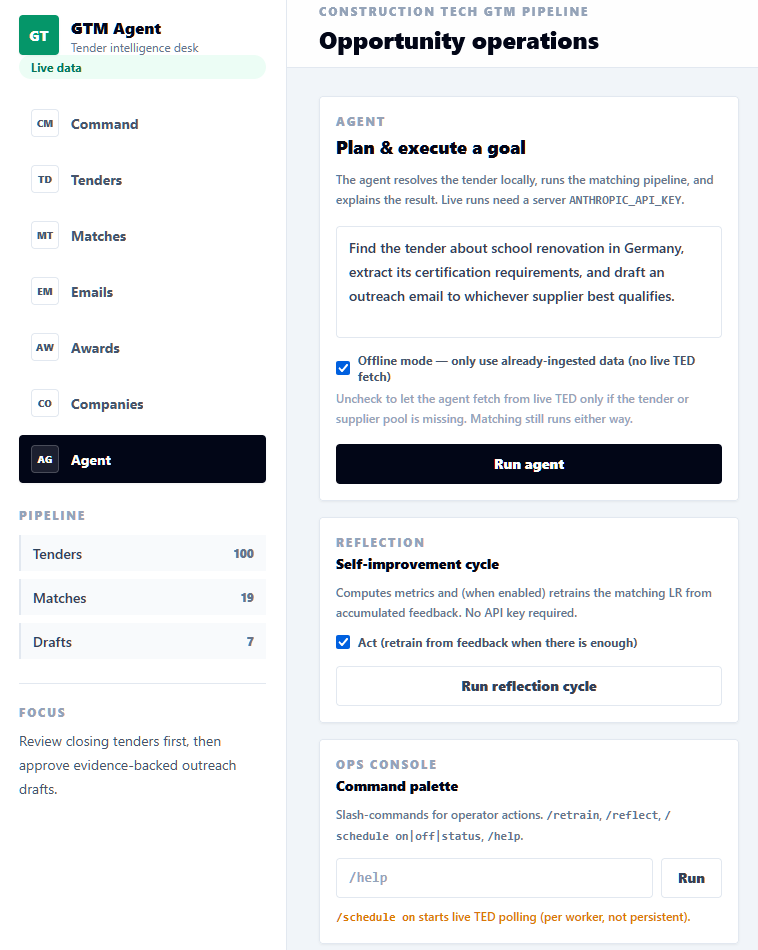
\includegraphics[height=8.5cm]{Agent-mode.png}\hspace{3mm}%
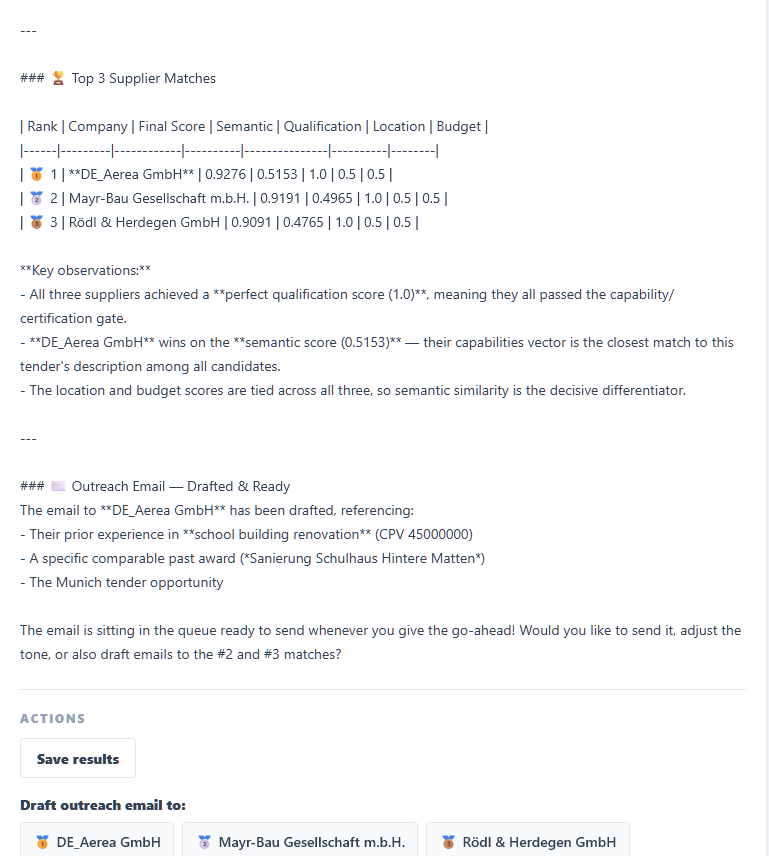
\includegraphics[height=8.5cm]{Agent-mode(Summary-EmailDraft).png}
\caption[Agent mode]{Ask in plain words: the assistant runs the steps live (left) and returns a ranked result (right).\label{fig:agent}}
\end{figure}

\subsection{Agent mode for power users: Just say what you want}\label{agent-mode}

Prefer not to click around? Tell the built-in assistant, in plain words,
for example, \emph{``Find the tender about school renovation in Germany, extract its certification requirements, and draft an outreach email to whichever supplier best qualifies.''} It works through the steps for you and shows what it's doing as it
goes (Figure~\ref{fig:agent}). A few things make it easy to trust:

\begin{itemize}
\tightlist
\item
  \textbf{Name a tender any way you like}, by its title or its official TED notice
  number (for example 420398-2026). If several could match, it stops and asks you
  to pick one instead of guessing.
\item
  \textbf{It stays on your data.} An ``Offline mode'' toggle is on by default, so it
  only uses the tenders and companies already loaded and won't reach out to the internet.
\item
  \textbf{One-click follow-ups.} When it's done, \textbf{save the result} or
  \textbf{draft an email} to any of the top matches in a single click.
\end{itemize}


\section{A typical session (walkthrough)}\label{a-typical-session}

\begin{enumerate}
\def\labelenumi{\arabic{enumi}.}
\tightlist
\item
  Open the \textbf{Tenders} screen and spot \emph{``Czechia, carriageway
  resurfacing works, D11.''}
\item
  Open it and view the matches, the top results are genuine Czech road builders
  (EUROVIA, STRABAG, SWIETELSKY).
\item
  Open the top company to read why it fits and what it's based on.
\item
  Generate an email and review the draft, every claim traces back to a real
  source.
\item
  Edit, give it a thumbs-up, and you're done: a sourced lead and a ready email in
  under a minute.
\end{enumerate}

\section{Common questions}\label{faq}
\begin{itemize}
\tightlist
\item
  \textbf{Does GTM Agent send emails on its own?} No, it only writes drafts for you
to review. You're always in control.
\item
  \textbf{Where does the data come from?} Only from public EU tender records, no
private or personal data.
\item
  \textbf{Can it handle other languages?} Yes, it reads tenders in any EU language,
and writes each email in the tender's own language.
\item
  \textbf{What fields does it cover?} Building/construction and IT services to start,
and it can be set up for other fields.
\item
  \textbf{Can the assistant do things on its own?} Nothing surprising. It only uses
data already loaded, asks before acting when something is unclear, and never sends
an email by itself.
\end{itemize}




%=============================================================================
%  PART 2 — PROJECT MANAGEMENT REPORT
%=============================================================================
\part{Project Management Report}
% !TEX root = ../FinalReport.tex
\chapter{Project Management Report}

\section{Overall Project Vision}

\subsection{Problem}
In B2B sales for construction, infrastructure and IT/services projects, business
development teams spend significant time finding relevant tenders and identifying
plausible bidders. Public
contracts above the EU thresholds must be advertised Union-wide (Directive
2014/24/EU), which makes TED an exhaustive but very high-volume source.
Because TED does not reveal active bidders during the tendering phase, teams still
rely on manual portal searches, company research, and fragmented market knowledge,
leading to wasted effort, missed opportunities, and missed deadlines.

\subsection{Solution and Scope}
GTM Agent turns public TED data into actionable sales leads. The MVP focuses on
construction and IT/services tenders filtered by CPV codes, the EU's standard
procurement classification (Regulation (EC) No 2195/2002). It combines live
Contract Notices with historical Award Notices, using CPV, buyer, and budget
similarity to identify companies likely to bid on similar projects again.

\textbf{Key deliverables (in scope)}

\begin{enumerate}
\tightlist
\item Automated ingestion of TED contract notices and award notices, plus
  dossier-PDF download where the document is directly reachable.
\item Entity resolution of award winners into canonical company records.
\item A hybrid tender↔company matcher with explainable sub-scores.
\item Evidence-grounded, two-sided email generation (supplier + buyer).
\item A feedback capture and weight-retraining loop.
\item A Claude tool-use agent that plans and executes the pipeline from a
  natural-language goal.
\item A Vue web dashboard and a documented REST API.
\end{enumerate}

\textbf{Boundaries}

\begin{enumerate}
\tightlist
\item No credential-juggling scraping of authenticated buyer portals --- restricted
  dossiers are flagged for manual review rather than scraped (see the Safety report).
\item No translation layer --- multilingual content is handled natively by a
  multilingual embedding model rather than machine translation.
\item No authentication / multi-tenancy in Phase 1.
\item No automatic sending of emails --- drafts are produced for human review only.
\item Vision-LLM blueprint parsing and a Neo4j incumbency knowledge graph are
  catalogued as \textbf{Future Work}, not committed to the MVP.
\end{enumerate}

\subsection{Success criteria}
The core evaluation method of the project is backtesting. For the historical tender,
the system goes back to its release time, runs the matcher only with the information
available at that time, and observes the ranking of the real winning company in the
results. The stage target is: Top-10 hit-rate ≥ 50\% in the MVP stage, increase to
≥ 65\% after mid-term, and the final target is ≥ 75\%. Because the implemented
backtest reports hit-rates only up to Hit@5, these stage targets were operationalised
as Top-1 ≥ 25\% and Top-5 ≥ 55\%. The final model meets both (Hit@1 44.2\%,
Hit@5 57.6\% on 500 held-out awards; full figures and their limits are discussed in
Part~\ref{part:safety}); the aspirational Top-10 ≥ 75\% was not separately measured
and no claim is made about it.

\section{Project Timeline}

\subsection{Gantt Chart}

The project is organised into eleven phases over twelve teaching weeks, clustered
into five workstream categories: Ingestion, Understanding \& Matching, Generation \&
Agent, Frontend \& Demo, and Documentation \& Evaluation. Figure~\ref{fig:timeline}
shows how the workstreams overlap and where the milestones fall.

\begin{figure}[!ht]
\centering
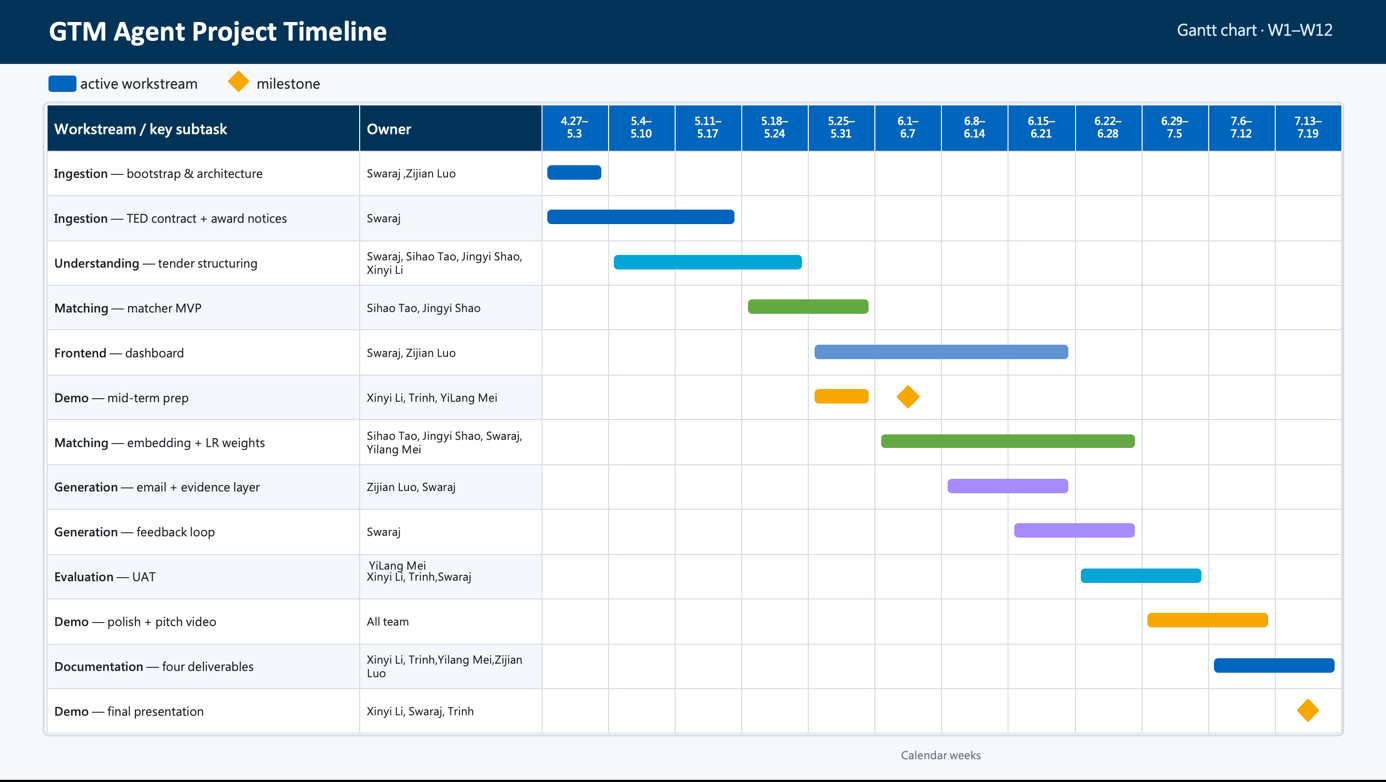
\includegraphics[width=0.98\linewidth]{pm_timeline.png}
\caption[Project timeline]{Project timeline (workstreams and milestones over teaching
weeks W1--W12).\label{fig:timeline}}
\end{figure}

\subsection{Milestones}

The roadmap in Figure~\ref{fig:milestones} groups the same twelve weeks into three
stages. It moves from data ingestion and MVP construction to matching, email, and
retraining features. The final stage covers UAT, documentation, presentation, and
submission.

\begin{figure}[!ht]
\centering
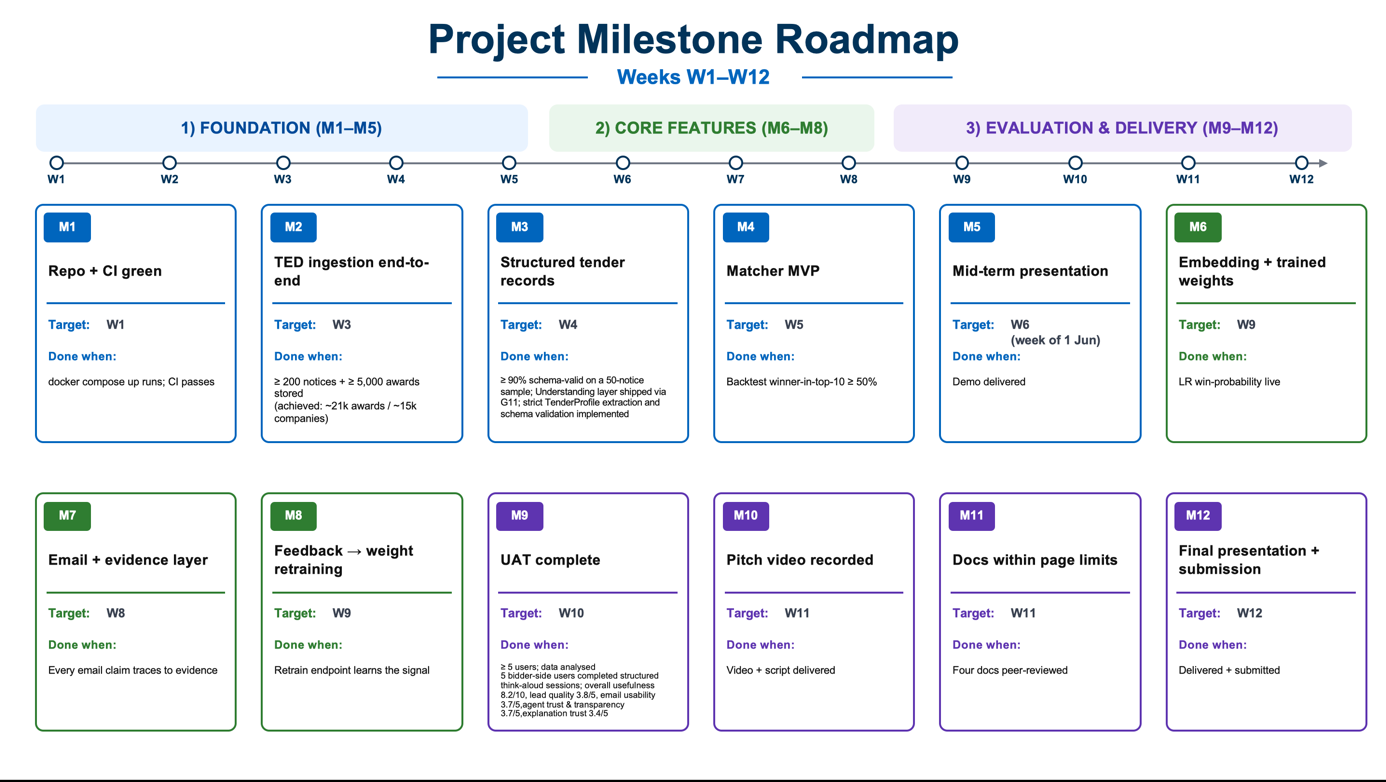
\includegraphics[width=0.98\linewidth]{pm_milestone.png}
\caption[Milestone roadmap]{Milestone roadmap across the three project
stages.\label{fig:milestones}}
\end{figure}

\section{System Architecture}

GTM Agent is organised into seven sub-systems, spanning data ingestion, storage,
matching, evidence-grounded generation, and agent orchestration.
Figure~\ref{fig:architecture} shows how they connect, and the paragraphs below
describe each in turn.

\begin{figure}[!ht]
\centering
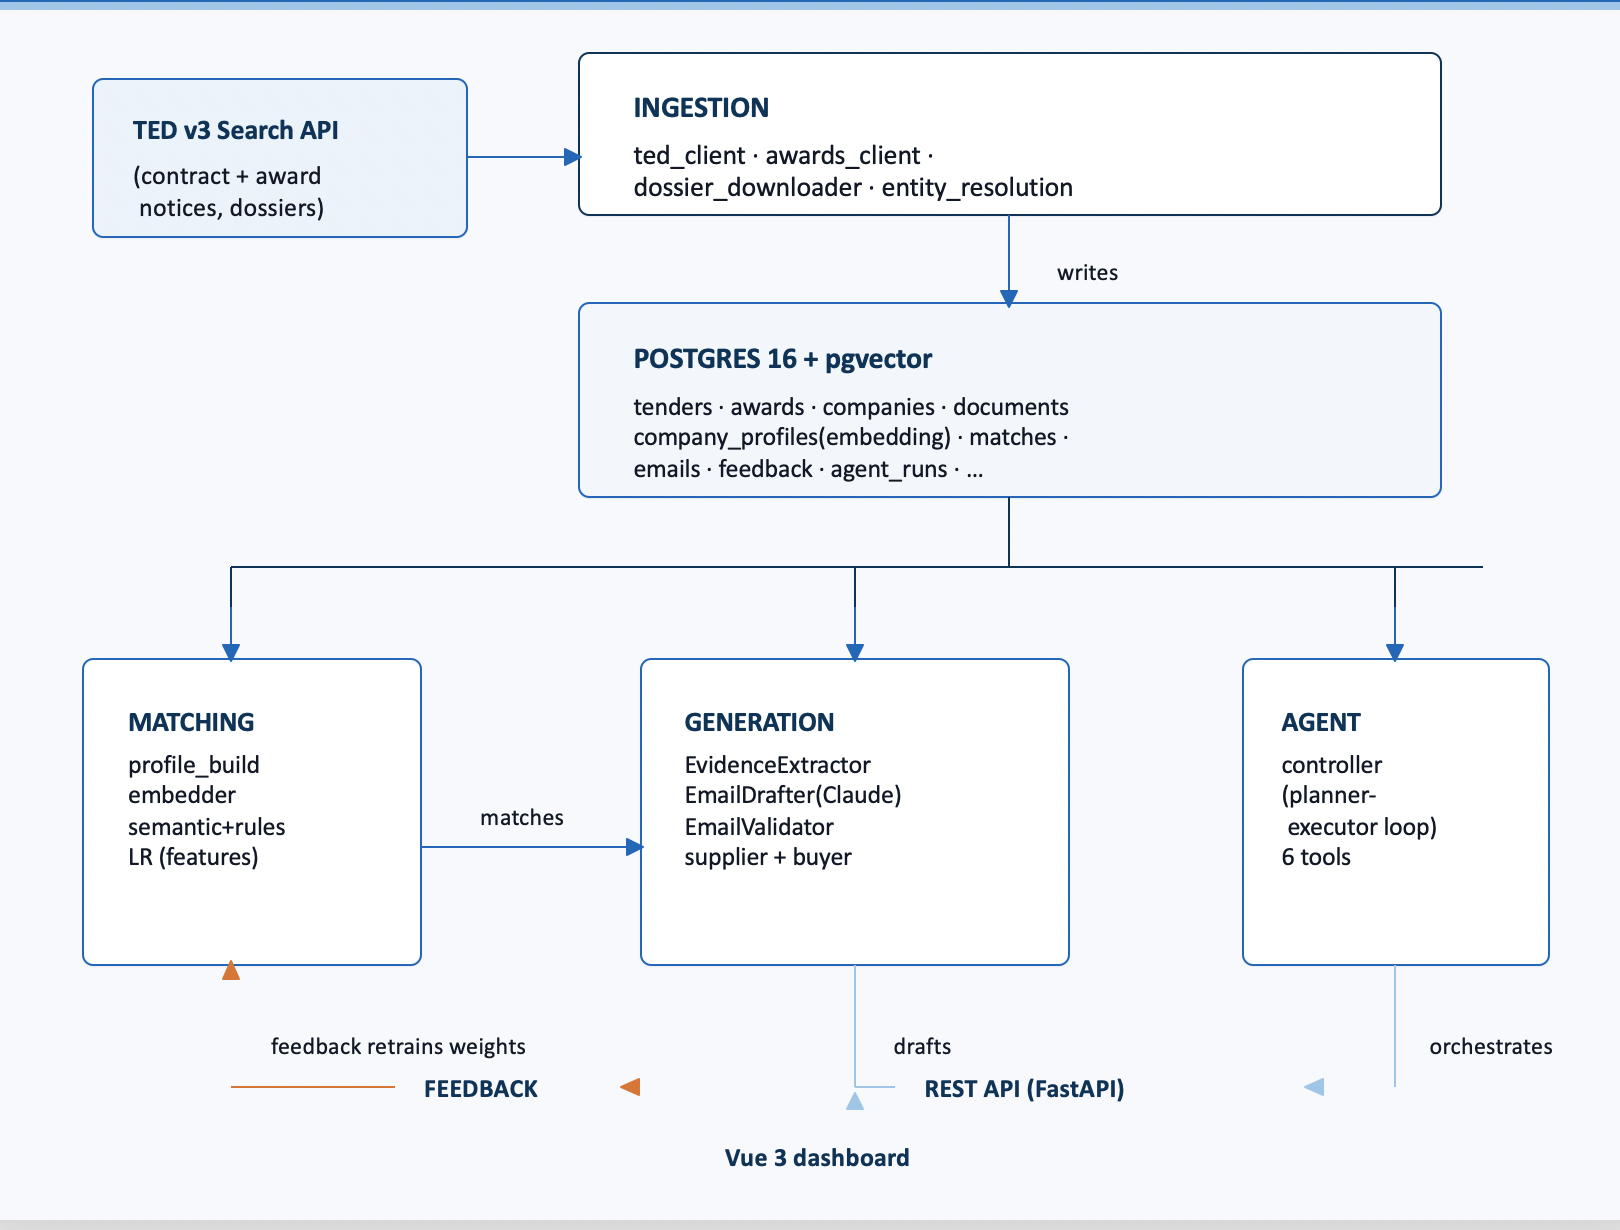
\includegraphics[width=0.90\linewidth]{pm_architecture.png}
\caption[System architecture]{System architecture: ingestion, storage, matching,
generation, and agent.\label{fig:architecture}}
\end{figure}

\subsection{Sub-systems}

\textbf{1. Ingestion.} The module retrieves live Contract Notices and historical
Award Notices through the TED v3 Search API and stores them in PostgreSQL.
Accessible dossier PDFs are downloaded, validated, deduplicated with SHA-256, and
converted to text. Command-line jobs include retry and rate-limit handling to
improve reliability.

\textbf{2. Entity Resolution.} The module standardizes company names by normalizing
capitalization, punctuation, and legal suffixes. It matches firms primarily through
reliable identifiers such as tax IDs and otherwise uses canonical names, while
filtering invalid identifiers to prevent incorrect merges.

\textbf{3. Tender Understanding.} The module converts notice and dossier content
into a structured TenderProfile, covering fields such as budget, deadline, CPV codes,
qualifications, and technical requirements. Outputs follow a strict JSON schema and
are validated through CPV repair, budget checks, and deduplication.

\textbf{4. Matching.} The matching module builds company profiles from historical
awards, including capabilities, embeddings, project scale, and location. It then
filters candidates by CPV, region, budget, and qualifications before using semantic
features and a Logistic Regression model whose output is calibrated to a usable win
probability (Niculescu-Mizil \& Caruana, 2005), implemented in scikit-learn
(Pedregosa et al., 2011).
Sub-scores and explanations show users why each company is ranked.

\textbf{5. Generation.} The system generates supplier outreach emails and buyer
tender digests. An Evidence Extractor supplies verified facts, and Claude drafts the
email under evidence constraints, with a deterministic template as fallback. An Email
Validator rejects unsupported claims, and all drafts require user review before
sending.

\textbf{6. Agent.} The Agent uses Claude's tool-use capability to turn
natural-language goals into executable steps, including data retrieval, matching,
email drafting, and read-only database queries. A planner--executor workflow streams
each step to the interface. For safety, write tools default to dry-run mode, database
access is limited to read-only SELECT queries, and external requests are strictly
bounded.

\textbf{7. API and frontend.} The FastAPI backend provides REST endpoints for
tenders, awards, companies, matches, emails, feedback, and Agent functions, with
automatic OpenAPI documentation. The Vue 3 frontend supports tender browsing,
candidate review, weight adjustment, score explanations, and email approval. Sample
data is used as a fallback when the backend is unavailable.

\subsection{Data model (selected)}
The system stores tenders, awards, companies, profiles, matches, emails, feedback,
and Agent runs in a unified PostgreSQL schema. \texttt{company\_profiles} uses
pgvector to store 384-dimensional embeddings for similarity matching, while a general
embeddings table supports future models. Company master data and capability profiles
are kept separately because they have different sources and update cycles. Full schema
details are documented in \texttt{docs/Database\_Explanation.md}.

\section{Method}

\subsection{Methodological principles}
Three principles shaped every technical decision:

\begin{enumerate}
\tightlist
\item \textbf{Classical ML over LLM where one exists.} The ranking of the matches is
  done by embeddings and logistic regression, not by asking an LLM, giving
  reproducible and explainable scores.
\item \textbf{Open-source, locally-run embedding models.} The most frequent operation
  in the pipeline --- semantic similarity between a tender's requirements and a
  company's portfolio --- runs locally, so there is no per-query API cost.
\item \textbf{Constrain the LLM to extraction and drafting.} The LLM never does
  free-form ranking or makes unverified factual claims. Because fluent but
  unsupported output is a known failure mode of generative models (Ji et al., 2023),
  restricting the model to evidence-backed information is a design constraint rather
  than a stylistic preference.
\end{enumerate}

\subsection{Hybrid matching method}
The core engineering of GTM Agent is its hybrid matching pipeline, which decomposes
the problem into independent layers, each using the right tool
(Table~\ref{tab:layers}).

\begin{table}[!ht]
\centering
\caption[Hybrid matching layers]{Hybrid matching: each layer uses the right
tool.}\label{tab:layers}
\renewcommand{\arraystretch}{1.2}
\begin{tabular}{@{}ll@{}}
\toprule
\textbf{Layer} & \textbf{Tool} \\
\midrule
Structured field extraction & LLM (Claude) \\
Semantic similarity & Open-source sentence embeddings \\
Budget / location / qualification & Deterministic rules \\
Weight fusion & Logistic regression \\
\bottomrule
\end{tabular}
\end{table}

\textbf{1) Hard disqualification.} Claude extracts structured fields from the tender
and company sources but does not rank yet. Before any scoring, a disqualifier removes
clearly ineligible candidates using deterministic filters (blacklisting, geographic
eligibility, company size versus budget tier, or tender-specific exclusions), so the
more expensive scoring steps only run on cleaner shortlists.

\textbf{2) Semantic similarity.} For each surviving candidate, a sentence embedding
model converts each text into a fixed-length vector, positioning semantically related
texts close together and making similarity computable as a cosine distance rather than
as word overlap (Reimers \& Gurevych, 2019). The model used is a distilled MiniLM
(Wang et al., 2020) whose multilingual variant is trained so that a sentence and its
translation land at the same point in the vector space (Reimers \& Gurevych, 2020).
That property is what lets a Czech tender be matched against a German company profile
without a translation step --- necessary for a platform like TED.

\textbf{3) Rule-based checks.} Budget overlap, geographic fit, and CPV qualification
are covered by deterministic sub-scores, because they involve structured data with
unambiguous answers: budget fit (after FX normalisation to EUR), geographic fit
(NUTS regions, Regulation (EC) No 1059/2003), and hierarchical CPV qualification
(an exact 8-digit CPV scores 1.0).

\textbf{4) Logistic-regression weight fusion.} A logistic regression, trained on
historical award notices with the ground truth ``did this company actually win?'',
combines ten features into a calibrated win probability; its coefficients give a
clear per-feature explanation. A feedback loop retrains it on thumbs-up/thumbs-down
pairs, storing a lasting feature snapshot with each feedback row so re-matching never
destroys training data.

\subsection{Prompt Engineering}
GenAI is used in three places, each with a deliberate prompting strategy.

\textbf{Structured field extraction.} A chain-of-thought-style prompt, following the
step-by-step decomposition principle of Wei et al.\ (2022), asks the model to describe
the type of section it is reading, list candidate fields, and produce a JSON fragment
following a strict schema. Only the JSON is processed and
checked; shape failures are rejected. The model is prompted in English while
foreign-language source text is included verbatim, using its multilingual reading
ability without a translation step.

\textbf{Evidence-grounded email drafting.} A two-step pattern: a deterministic
extractor first builds the evidence list (TED ID, CPV codes, deadline, match scores,
company facts); the model then receives only that evidence and is instructed to add no
claim outside it. Output is post-validated, and any unsupported entity or claim flags
the draft for review rather than sending. The prompt also tells the model to match the
tender's language automatically.

\textbf{Agent orchestration.} The agent follows the reason-then-act pattern of Yao
et al.\ (2023): it alternates a short planning step with a tool call and feeds the
tool result back before deciding the next step. A planner--executor system prompt
defines the goal, the tool set (as JSON schemas), and safety constraints (DB-first resolution,
offline-by-default ingest, read-only SQL, \texttt{ask\_user} for ambiguity). Tool
definitions and the system prompt stay stable across turns to benefit from prompt
caching, and messages persist to \texttt{agent\_sessions} so a paused run resumes
exactly where it left off.

\section{Technology Used}

The stack is a Python/FastAPI backend, a PostgreSQL + pgvector database, and a Vue 3
frontend, with open-source models for ranking and Claude for generation and the agent
(Table~\ref{tab:tech}).

{\small\renewcommand{\arraystretch}{1.1}%
\begin{xltabular}{\textwidth}{@{}>{\raggedright\arraybackslash}p{2.5cm} >{\raggedright\arraybackslash}p{4.9cm} >{\raggedright\arraybackslash}X@{}}
\caption[Technology stack]{Technology stack.}\label{tab:tech}\\
\toprule
\textbf{Layer} & \textbf{Technology} & \textbf{Notes}\\
\midrule
\endfirsthead
\toprule
\textbf{Layer} & \textbf{Technology} & \textbf{Notes}\\
\midrule
\endhead
\bottomrule
\endlastfoot
Language / runtime & Python 3.11 & Pinned for dependency compatibility\\
HTTP framework & FastAPI 0.115 & First-class Pydantic v2 + OpenAPI\\
Validation & Pydantic v2 & Strict schema enforcement\\
ORM / migrations & SQLAlchemy 2.0 / Alembic & Typed \texttt{Mapped[]} API\\
Database & PostgreSQL 16 + pgvector & Single schema; vector similarity in-DB\\
HTTP client & httpx (+ truststore) & \texttt{requests} banned by spec\\
PDF text & PyMuPDF & Dossier extraction\\
Embeddings & sentence-transformers: paraphrase-multilingual-MiniLM-L12-v2 (384-d), CPU-only & Multilingual MiniLM; lazy-loaded\\
Classical ML & scikit-learn + joblib & Trained logistic-regression matcher (calibrated win-probability)\\
LLM & Anthropic Claude (\texttt{claude-sonnet-4-6}) & Agent, reflection, email drafting\\
Scheduler & APScheduler (in-process) & Opt-in cron loop (ingest + reflect); runtime on/off/status toggle\\
Frontend & Vue 3 / TypeScript / Vite 5 / Pinia / Tailwind & Three-column dashboard\\
CI & GitHub Actions & pytest · lint+build · migration smoke\\
Containerisation & Docker Compose & db + backend + frontend\\
\end{xltabular}}

\section{Current Progress and Future Plans}

Every planned MVP component is implemented, and the components on the critical path
have been smoke-tested against live TED data; Table~\ref{tab:status} summarises their
status, followed by known limitations and future work.

{\small\renewcommand{\arraystretch}{1.1}%
\begin{xltabular}{\textwidth}{@{}>{\raggedright\arraybackslash}p{5.2cm} >{\raggedright\arraybackslash}X@{}}
\caption[Component status]{Component status.}\label{tab:status}\\
\toprule
\textbf{Component} & \textbf{Status}\\
\midrule
\endfirsthead
\toprule
\textbf{Component} & \textbf{Status}\\
\midrule
\endhead
\bottomrule
\endlastfoot
Repo scaffold, schema, CI & Done\\
TED contract-notice ingestion & Done: CPV-filtered, live-verified\\
Award back-fill + entity resolution & Done: \textasciitilde21k awards / \textasciitilde15k companies cleaned and stored; 24-month back-fill planned\\
Dossier downloader + ingestion CLI & Done (scoped): ingestion-only utility; thin coverage\\
Understanding layer (Claude field extractor) & Done: tender profile persisted; soft fields only\\
Matching (hybrid + trained model) & Done: multilingual embeddings (MiniLM), rules, and a calibrated logistic regression; returns top-N with sub-scores; live-smoked\\
Ranking + explanations & Done: per-supplier sub-scores plus explanation; numbers only from \texttt{query\_db}, live score recalculation runs in the browser with no round-trip\\
Email generation (Claude) & Done: constrained generation only; all evidence validated and grounded; live-verified\\
Feedback capture + retraining & Done: feedback retrains the model\\
Scheduler (opt-in) + reflection loop & Done: reflections stored; runtime on/off/status control\\
Agent (DB-first, streaming, resumable, result actions) & Done: planner--executor loop, max 20 turns, every step streamed live; pauses for user input and resumes from the saved session; live-smoked\\
Ops command console & Done: \texttt{/retrain}, \texttt{/reflect}, \texttt{/schedule}, \texttt{/help}\\
REST API (7 routers) + Vue dashboard (7 views) & Done: browse tenders, open detail pages, inspect recommendations, approve and send email; sample-data fallback\\
ML training dataset export + retrain on 80\% of awards & Done: 16,812 training awards\\
\end{xltabular}}

\textbf{Limitations and future plans.} Company profiles come from award history only,
so the supplier pool is limited to companies that have won a listed EU tender;
per-portal dossier scraping is prepared but not yet built, and the external match
fallback (suggesting and scraping websites when no strong internal match exists) is
out of scope. This fixed supplier pool also explains why the certification
disqualifier, although built and linked to the extraction layer, stays inert in
production: the award data carries no supplier-certification field. Because TED
publishes no supplier email addresses, supplier recipients are website-derived and
marked unverified rather than fabricated, consistent with the rule never to create
information it cannot trace to a source.

Three UAT interface requests remain future work at the presentation layer (a city
field in the detail view, a company-website link in the email and detail views, and
shorter tender titles); they were deferred to focus on the agent work. Match alerts
and competitor analysis are also valuable requests that reuse existing components ---
alerts as a scheduled query over stored matches, competitor analysis as aggregation
over already-ingested award history. Finally, vision-model blueprint parsing, a Neo4j
incumbency knowledge graph, and an embedding ensemble (adding \texttt{all-mpnet-base-v2}
and \texttt{multilingual-e5-large}) are catalogued but not committed.

% The per-chapter reference list was consolidated into the report-wide References
% chapter at the end of the document (chapters/references.tex).


%=============================================================================
%  PART 3 — USER ACCEPTANCE TESTING REPORT
%=============================================================================
\part{User Acceptance Testing Report}\label{part:uat}
% !TEX root = ../FinalReport.tex
\chapter{User Acceptance Testing Report}

\section{Target Users Research}

\subsection{Target users}
This UAT invited a total of five bidder-side users from the transportation, energy,
and construction industries. Their positions include Tender Specialist, Project
Development, Sales Support, Business Development, and company CEO. The first four are
direct daily users of the system, while the CEO represents the manager who ultimately
decides whether the enterprise will participate in a given tender.

\subsection{Reasons for choosing these users}
These users are directly related to the core usage scenarios of GTM Agent and can
judge, from an actual business perspective:

\begin{enumerate}
\tightlist
\item whether the company recommended by the system is a reasonable potential bidder;
\item whether the matching score and explanation are credible enough;
\item whether the weight adjustment is in line with business judgment;
\item whether the operation process of the Agent is transparent and controllable.
\end{enumerate}

\subsection{Advantages and limitations of user research}
Testing with real industry personnel yields direct feedback with business context and
checks whether the product really solves the problem of bidding discovery and
potential-company screening. The participants' positions are diverse, including both
daily executives and decision-makers. The limitation is that the sample size is only
five people, so no general statistical inference can be made; participants' familiarity
with the bidding process also varies. Five participants are a common working minimum
for qualitative usability testing (Nielsen \& Landauer, 1993), but that argument
concerns the discovery of interface problems, not the estimation of population means:
the rating averages below are indications, not measurements. In addition, the test
uses system data and
scenarios prepared by the team, not the real private data of the participants'
enterprises.

\section{User Testing Design}

\subsection{Test method}
Each participant completes a structured think-aloud session (Ericsson \& Simon, 1993),
verbally expressing their judgments, confusions, and expectations while working, so
that reasoning is captured as it happens rather than reconstructed afterwards. The test
combines task scenarios with a
post-test questionnaire: first observing whether the user can complete the core
process, then collecting feedback through scale scoring and open-ended questions. The
UAT script is in Appendix A.

\subsection{Testing tasks}
Participants complete three core tasks in turn:

\begin{enumerate}
\tightlist
\item \textbf{Looking for candidate companies.} Choose a tender, check the companies
  recommended by the matcher, and judge whether the top-ranked company is a credible
  potential bidder.
\item \textbf{Adjust the matching weight.} Use the weight sliders to adjust factors
  such as semantic matching, budget, region, and qualification, and observe whether
  the ranking changes in real time as expected.
\item \textbf{Generate and review emails.} Generate an evidence-based outreach email
  for a candidate company, check whether it relates to the tender and company
  background, and judge whether it is usable after minor edits.
\end{enumerate}

\subsection{Evaluation indicators}
The test mainly evaluates: task completion, task time, lead quality (are the
recommended companies reasonable), explanation trust (does the user understand and
trust the ranking), email usability (usable after minor edits), agent trust and
transparency, overall usefulness / recommendation intention, and open feedback
(obstacles encountered and desired features). Scale items use 1--5 Likert points
(Likert, 1932), and the overall recommendation item uses the 0--10 Net Promoter
question (Reichheld, 2003).

\section{Analysis and Evaluation of Results}

\subsection{Main results}
The five participants rated overall usefulness at 4.1/5 in the post-test questionnaire
and willingness to recommend at 8.2/10; lead quality at 3.8/5, with email usability and
agent trust both at 3.7/5. Explanation trust had the lowest score, 3.4/5. Every
participant's recommendation intention was at least 7/10, indicating overall
recognition of the system's value. Scored as a Net Promoter Score (two promoters, three
passives, no detractors) the result is $+40$, although with five participants a single
detractor would move that by twenty points. All five reached the end of the core
workflow: two completed it fully and independently, while the other three needed minor
facilitator guidance and are recorded as partial completions. Time on task ranged from
18 to 28 minutes, with the fastest completions by the most frequent TED users.
Figures~\ref{fig:uat-participants} and~\ref{fig:uat-scores} report the per-participant
results and the resulting means.

\begin{figure}[!ht]
\centering
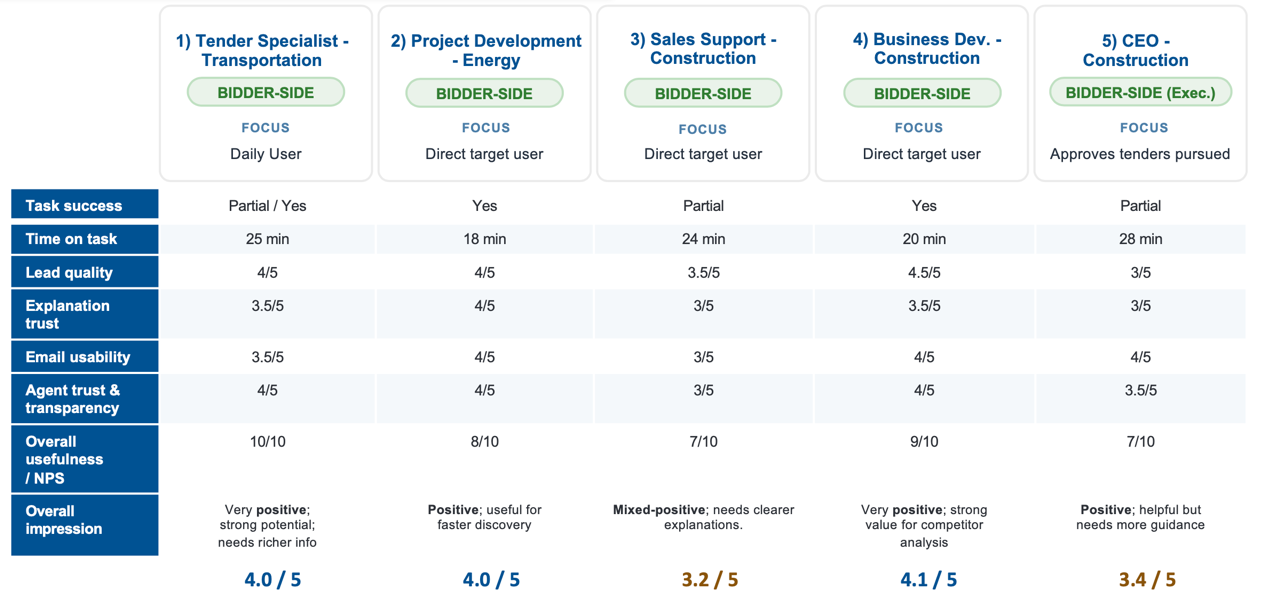
\includegraphics[width=0.78\linewidth]{uat_participants.png}
\caption[Per-participant UAT results]{Per-participant results; scale items use 1--5,
the recommendation item 0--10.\label{fig:uat-participants}}
\end{figure}

\begin{figure}[!ht]
\centering
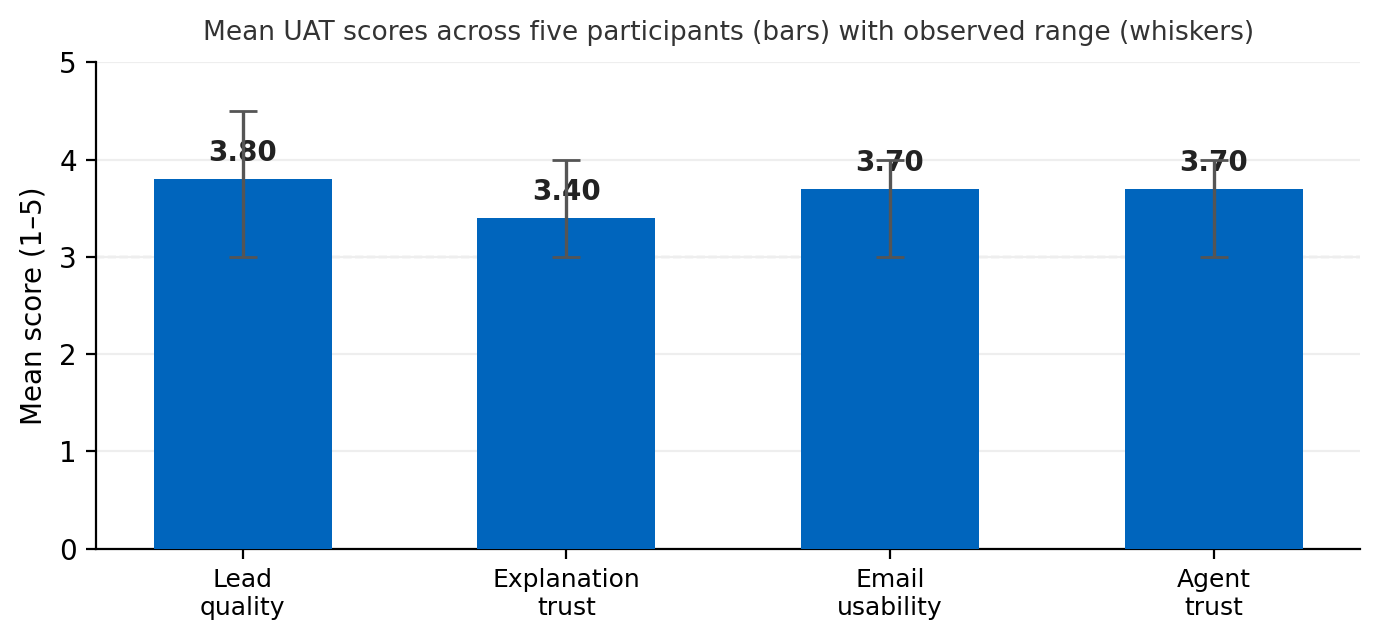
\includegraphics[width=0.55\linewidth]{uat_scores.png}
\caption[Mean UAT scores]{Mean UAT scores, whiskers showing the observed
range.\label{fig:uat-scores}}
\end{figure}

\subsection{Core findings}
Users generally believe the system reduces the time spent manually browsing TED and
searching for potential companies, and that the recommendations carry a certain
business rationality. However, users' understanding of ``why the ranking changes'' is
weak, so the natural-language explanation still needs strengthening --- reflected in the
lowest mean score, explanation trust (3.4/5). Participants could nonetheless read the
named ranking factors (semantic match, budget, region, qualification). All participants
also asked that the email directly present the tender's core information, such as
budget, deadline, and location.

\subsection{Feedback processing}
In response to concerns about insufficient email information, the team added a tender
summary block with budget, deadline, and location, removing the need to return to the
tender page before sending. The Agent Q\&A was also expanded so users can query tender,
company, and matching data, not just request recommendations. Requests that could not
be met within the MVP --- city fields, company-website links, shorter tender titles,
match alerts, and competitor analysis --- were recorded as future work.

\subsection{Conclusion}
UAT shows that GTM Agent does address the practical problems of target users in
discovering bidding opportunities, screening candidate companies, and preparing initial
outreach. Users most valued the efficiency gain and the lead quality, but trust in the
ranking explanation remains the most important area for improvement. Subsequent
development should therefore prioritise the natural-language explanation, supplement
key tender and company information, and retain human review of emails and results.


%=============================================================================
%  PART 4 — GENAI SAFETY AND REFLECTION REPORT
%=============================================================================
\part{GenAI Safety and Reflection Report}\label{part:safety}
% !TEX root = ../FinalReport.tex
\chapter{GenAI Safety and Reflection Report}

\textit{Scope and evidence.} GTM Agent supports EU-procurement business development by
ingesting public TED notices and historical awards, ranking candidate suppliers, and
drafting outreach for human review. This report draws on the implemented system, the
ranking backtest, and a five-participant user-acceptance test (UAT), and keeps
implemented controls, evaluation findings, and residual boundaries distinct so that
design intent is not mistaken for evidence of safety.

\section{System boundary and evaluation lens}

\textbf{Where GenAI is used.} GTM Agent does not hand the whole decision chain to one
model. GenAI performs three bounded tasks: extracting soft fields into a schema,
drafting emails from a structured evidence object, and orchestrating a restricted tool
set. Supplier ranking stays outside the generative path (multilingual embeddings,
deterministic rules, and logistic regression), keeping the recommendation measurable
and explainable while confining the model to language and orchestration.

\textbf{What counts as evidence.} The vision specified a two-sided MVP, a hybrid
matcher, feedback and retraining, reviewable drafts, an agent, a ranking backtest, and
UAT. The final model, trained on the earlier 16,812 awards and evaluated on 500
chronologically later held-out awards, reached Hit@1 / Hit@3 / Hit@5 of
44.2\% / 54.0\% / 57.6\%, meeting the Top-1 ($\geq25\%$) and Top-5 ($\geq55\%$) targets.
Two boundaries qualify that number. The test set is restricted to tenders whose winner
is a company the system already knows, so it measures ranking, not coverage of unknown
firms; but the winner is not exempted from the hard filter, and the 26.6\% of cases in
which the filter removes it are counted as misses rather than excluded. Hit@10 and MRR
were not reported, so no claim is made about them.

\section{Safety of GenAI}

Risks arise from generated outputs, agent actions, untrusted inputs, and operation.

\textbf{Factual integrity of emails.} Emails are where generated content reaches users,
so an inaccurate claim about a supplier, a deadline, or prior work is the primary
output risk --- and fluent, confident, unsupported text is a well-documented failure
mode of generative models rather than an occasional defect (Ji et al., 2023). The
system assembles the tender record, supplier profile, scores, match
explanation, and document excerpts, then asks Claude to draft from that evidence alone;
if the model call, JSON parsing, or validation fails, a deterministic template is built
from the same evidence. Every output is stored as a \texttt{draft} and nothing is sent
automatically. These measures limit unsupported content but do not verify every
statement: the current \texttt{EmailValidator} checks subject, body, and length, not
each claim against a source, so human review remains necessary, and a production
version should require every claim to resolve to an identifiable source.

\textbf{Agent authority.} An early version treated \texttt{dry\_run} as a safety
switch, but it blocked database writes without blocking network calls, so a routine
request could start costly TED polling and document scanning. The revised agent makes
dry-run network-free, resolves tenders from the local database by default, and removes
bulk dossier download entirely. Live ingestion is bounded (look-back window, row limit,
once per goal, with an extra condition on award ingestion); the database tool is
read-only (write verbs blocked, row cap, read-only connection); and \texttt{ask\_user}
pauses on ambiguity rather than guessing. The operator console (scheduler, retraining)
is still unauthenticated and would need access control and an audit policy before
deployment.

\textbf{Untrusted inputs, provenance, and privacy.} Tender and dossier text is
attacker-influenced and may carry instructions unrelated to the task --- the indirect
prompt-injection channel described by Abdelnabi et al.\ (2023), in which the payload
reaches the model through retrieved content rather than through the user's own turn.
Schema-constrained extraction, evidence-bounded drafting, restricted tools, and
downstream validation limit --- though do not eliminate --- that channel: untrusted
text cannot alter the deterministic ranking path or gain general write access. The data
is public TED and award records, not private customer data; raw payloads, the evidence
object, and each document's source URL and content hash are retained; files behind
buyer-portal logins are marked \texttt{restricted} rather than scraped. Two
qualifications follow. Supplier contact addresses derived from company websites are
still personal data under Regulation (EU) 2016/679 even though their source is public,
so deployment would need a lawful basis, retention periods, role-based access, and a
privacy review. And because the system generates text that is sent to people on the
system's suggestion, the transparency and human-oversight duties of Regulation (EU)
2024/1689 are the relevant compliance frame for a production version, even though a
lead-generation assistant is not itself a high-risk system under that regulation.

\textbf{Reliability, cost, and fairness.} Rate limiting and retries bound TED
ingestion, local embeddings cut external calls, and a train--serve feature-contract
test guards the deployed matcher, with the deterministic email fallback as an explicit
degradation path. Reliability is not fairness, however: award-history training can
entrench incumbents, and although component scores and adjustable weights make the
basis of a recommendation visible, they do not remove that advantage. With no fairness
metric yet reported, future evaluation should measure ranking quality for smaller and
newer suppliers, not only the recovery of past winners; the ranked group-fairness
criterion of Zehlike et al.\ (2017), which constrains the representation of a protected
group within every prefix of a top-\textit{k} list, is a concrete candidate measure for
that, with firm age or size as the grouping attribute.

\section{Lessons learned and reflection}

\textbf{Delivery versus evidence.} The MVP integrated ingestion, entity resolution,
hybrid matching, evidence-backed drafting, feedback and retraining, the agent, an API,
and a dashboard, but a component existing does not by itself prove product value. The
backtest gives quantitative evidence for the matcher and UAT adds workflow-level
evidence; together they describe completion better than a checklist.

\textbf{What the ranking KPI teaches.} The matcher met its Top-1 and Top-5 targets, yet
raising the training share from 50\% to 80\% did not improve Hit@3 (54.8\% to 54.0\%).
The two runs use different held-out slices, so this is not a controlled comparison and
the roughly one-point difference is within noise; the reading we take from it is
therefore modest --- more data of the same kind did not move the metric. That points to
a representation limit rather than too few examples, since capability profiles are built
from thin award-history text. Enriching those profiles or adding an embedding ensemble
is the more promising direction, and a controlled ablation on a fixed slice would be
needed to confirm it.

\textbf{What the UAT teaches.} Where the backtest asks whether the system retrieves the
known winner, UAT asks whether users can interpret and act on the result. Five
bidder-side participants from transportation, energy, and construction completed
think-aloud sessions covering candidate discovery, weight adjustment, and email
drafting; the full per-participant results are in Part~\ref{part:uat},
Figure~\ref{fig:uat-participants}. Perceived lead quality (3.8/5) exceeded explanation
trust (3.4/5): users saw the business value of the candidates but not always why each
ranked where it did. Showing a score is not the same as explaining it, so a future
interface should tie each recommendation to its CPV, geographic, budget, and semantic
evidence. With only five participants these are design priorities, not population-level
effects.

\textbf{Practices that worked, and what to change.} Assigning ranking to classical ML
and rules kept the path measurable and auditable, and repeated smoke tests against live
TED data caught defects (qualification scoring, budget normalisation) that an
interpretable architecture alone would not. The main organisational lesson is to agree
the interfaces between parallel workstreams early --- the in-app and standalone matchers
were unified late --- and to treat evaluation the same way: each KPI needs a fixed
dataset snapshot, an owner, a reproducible script, and a decision date from the start.
Scope discipline (deferring authenticated scraping, multi-tenancy, blueprint parsing,
and a knowledge graph) kept the MVP focused; the next stage should add claim-to-source
email checks, authenticated operator controls, a larger UAT with a human baseline, and
fairness analysis.

\section{How our understanding of GenAI changed, and conclusion}

The project reframed GenAI as a language-and-orchestration component bounded by evidence
objects, schemas, permissions, and user confirmation --- not a general decision-maker;
the dry-run incident showed that a control matters only when it blocks the exact action
that produces the risk. UAT separated usefulness from trust: a system can surface
valuable leads while users stay unsure of the reasoning, and a fluent draft can still
need factual review, so evaluating a GenAI application means weighing task completion,
ranking quality, factual support, user understanding, operational limits, and
auditability together. GTM Agent now forms an integrated MVP whose safety case rests on
evidence-constrained generation, human review, restricted tools, offline-by-default
agent behaviour, and traceable public data; the next stage should keep testing those
boundaries, especially email-claim verification, operator access control, and broader
user and fairness evaluation.


%=============================================================================
%  CLOSING — REFERENCES + GENAI USAGE ACKNOWLEDGMENT (whole submission)
%=============================================================================
\cleardoublepage
% !TEX root = ../FinalReport.tex
% Consolidated reference list for all four parts (APA 7th style).
% Every entry is cited at least once in Parts II--IV; the User Guide (Part I) is a
% user-facing document and deliberately carries no citations.
\chapter*{References}
\addcontentsline{toc}{chapter}{References}

\section*{Literature}

\refitem{Abdelnabi, S., Greshake, K., Mishra, S., Endres, C., Holz, T., \& Fritz, M.
(2023). Not what you've signed up for: Compromising real-world LLM-integrated
applications with indirect prompt injection. In \textit{Proceedings of the 16th ACM
Workshop on Artificial Intelligence and Security (AISec '23)} (pp.\ 79--90). ACM.
\url{https://doi.org/10.1145/3605764.3623985}}

\refitem{Ericsson, K. A., \& Simon, H. A. (1993). \textit{Protocol analysis: Verbal
reports as data} (Rev.\ ed.). MIT Press.}

\refitem{Ji, Z., Lee, N., Frieske, R., Yu, T., Su, D., Xu, Y., Ishii, E., Bang, Y. J.,
Madotto, A., \& Fung, P. (2023). Survey of hallucination in natural language
generation. \textit{ACM Computing Surveys, 55}(12), Article 248.
\url{https://doi.org/10.1145/3571730}}

\refitem{Likert, R. (1932). A technique for the measurement of attitudes.
\textit{Archives of Psychology, 22}(140), 1--55.}

\refitem{Niculescu-Mizil, A., \& Caruana, R. (2005). Predicting good probabilities with
supervised learning. In \textit{Proceedings of the 22nd International Conference on
Machine Learning (ICML '05)} (pp.\ 625--632). ACM.
\url{https://doi.org/10.1145/1102351.1102430}}

\refitem{Nielsen, J., \& Landauer, T. K. (1993). A mathematical model of the finding of
usability problems. In \textit{Proceedings of the INTERACT '93 and CHI '93 Conference
on Human Factors in Computing Systems} (pp.\ 206--213). ACM.
\url{https://doi.org/10.1145/169059.169166}}

\refitem{Pedregosa, F., Varoquaux, G., Gramfort, A., Michel, V., Thirion, B., Grisel,
O., Blondel, M., Prettenhofer, P., Weiss, R., Dubourg, V., Vanderplas, J., Passos, A.,
Cournapeau, D., Brucher, M., Perrot, M., \& Duchesnay, É. (2011). Scikit-learn: Machine
learning in Python. \textit{Journal of Machine Learning Research, 12}, 2825--2830.}

\refitem{Reichheld, F. F. (2003). The one number you need to grow. \textit{Harvard
Business Review, 81}(12), 46--54, 124.}

\refitem{Reimers, N., \& Gurevych, I. (2019). Sentence-BERT: Sentence embeddings using
Siamese BERT-networks. In \textit{Proceedings of the 2019 Conference on Empirical
Methods in Natural Language Processing and the 9th International Joint Conference on
Natural Language Processing (EMNLP-IJCNLP)} (pp.\ 3982--3992). Association for
Computational Linguistics. \url{https://doi.org/10.18653/v1/D19-1410}}

\refitem{Reimers, N., \& Gurevych, I. (2020). Making monolingual sentence embeddings
multilingual using knowledge distillation. In \textit{Proceedings of the 2020
Conference on Empirical Methods in Natural Language Processing (EMNLP)} (pp.\
4512--4525). Association for Computational Linguistics.
\url{https://doi.org/10.18653/v1/2020.emnlp-main.365}}

\refitem{Wang, W., Wei, F., Dong, L., Bao, H., Yang, N., \& Zhou, M. (2020). MiniLM:
Deep self-attention distillation for task-agnostic compression of pre-trained
transformers. In \textit{Advances in Neural Information Processing Systems 33}
(pp.\ 5776--5788). Curran Associates.}

\refitem{Wei, J., Wang, X., Schuurmans, D., Bosma, M., Ichter, B., Xia, F., Chi, E. H.,
Le, Q. V., \& Zhou, D. (2022). Chain-of-thought prompting elicits reasoning in large
language models. In \textit{Advances in Neural Information Processing Systems 35}
(pp.\ 24824--24837). Curran Associates.}

\refitem{Yao, S., Zhao, J., Yu, D., Du, N., Shafran, I., Narasimhan, K., \& Cao, Y.
(2023). ReAct: Synergizing reasoning and acting in language models. In \textit{The
Eleventh International Conference on Learning Representations (ICLR 2023)}.
\url{https://openreview.net/forum?id=WE_vluYUL-X}}

\refitem{Zehlike, M., Bonchi, F., Castillo, C., Hajian, S., Megahed, M., \&
Baeza-Yates, R. (2017). FA*IR: A fair top-\textit{k} ranking algorithm. In
\textit{Proceedings of the 2017 ACM Conference on Information and Knowledge Management
(CIKM '17)} (pp.\ 1569--1578). ACM. \url{https://doi.org/10.1145/3132847.3132938}}

\section*{Legal sources and data standards}

\refitem{Directive 2014/24/EU of the European Parliament and of the Council of 26
February 2014 on public procurement and repealing Directive 2004/18/EC. \textit{OJ}
L 94, 28.3.2014, pp.\ 65--242.}

\refitem{Regulation (EC) No 2195/2002 of the European Parliament and of the Council of
5 November 2002 on the Common Procurement Vocabulary (CPV). \textit{OJ} L 340,
16.12.2002, pp.\ 1--562.}

\refitem{Regulation (EC) No 1059/2003 of the European Parliament and of the Council of
26 May 2003 on the establishment of a common classification of territorial units for
statistics (NUTS). \textit{OJ} L 154, 21.6.2003, pp.\ 1--41.}

\refitem{Regulation (EU) 2016/679 of the European Parliament and of the Council of 27
April 2016 on the protection of natural persons with regard to the processing of
personal data and on the free movement of such data (General Data Protection
Regulation). \textit{OJ} L 119, 4.5.2016, pp.\ 1--88.}

\refitem{Regulation (EU) 2024/1689 of the European Parliament and of the Council of 13
June 2024 laying down harmonised rules on artificial intelligence (Artificial
Intelligence Act). \textit{OJ} L, 2024/1689, 12.7.2024.}

\refitem{Publications Office of the European Union. (n.d.). \textit{Tenders Electronic
Daily (TED) --- Supplement to the Official Journal of the EU.}
\url{https://ted.europa.eu}}


\cleardoublepage
% !TEX root = ../FinalReport.tex
% Appendix A belongs to Part III (User Acceptance Testing) but is placed after the
% References so that it does not count against that report's page budget.
\chapter*{Appendix A --- Evaluation Protocol (UAT Script)}
\addcontentsline{toc}{chapter}{Appendix A --- Evaluation Protocol (UAT Script)}

Supporting material for Part~\ref{part:uat} (User Acceptance Testing Report). Each
participant was assessed against the identical script and rating instrument.

\textbf{Background.} How many years have you worked with tenders?

\textbf{Scenario 1 --- Lead Discovery \& Justification.} \emph{Task:} find a tender in
your sector and identify the three most promising companies to approach.
\emph{Observed:} can they find the tender list, understand the rankings and score
explanations, and do they need help? \emph{Rating:} how plausible are these companies
as bidders for this tender? (1--5)

\textbf{Scenario 2 --- Weight Adjustment.} \emph{Task:} find the weighting controls,
adjust the ranking, review the new results, and explain whether the ranking changed as
expected. \emph{Observed:} can they discover the controls themselves and understand why
the ranking changed? \emph{Rating:} how much do you trust the ranking explanations?
(1--5)

\textbf{Scenario 3 --- Email Generation \& Verification.} \emph{Task:} generate an
outreach email for one company and review it before sending, checking supporting
evidence. \emph{Observed:} can they select a company, generate, and read the email; do
they understand where the evidence comes from; how much editing is required?
\emph{Rating:} rate the generated email (1--5) --- could you send it after only minor
edits?

\textbf{Overall survey.} How useful would this tool be for your work, and how much do
you trust the matching agent? (1--5) How likely are you to recommend it to a colleague?
(0--10)

\textbf{Open feedback.} What do you like most? What feature is missing? If you could
change one thing, what would it be? Would you actually use this tool, and why?

\textbf{Rating scales.} All per-scenario and agent-trust items use a 1--5 Likert scale
(1 = strongly negative \ldots{} 5 = strongly positive). The final recommendation item
uses a 0--10 (NPS-style) scale.


\cleardoublepage
\chapter*{Acknowledgment of GenAI Usage}
\addcontentsline{toc}{chapter}{Acknowledgment of GenAI Usage}

All four documents in this submission were written with the help of AI-based writing
assistants --- principally a Claude-based assistant, with OpenAI ChatGPT additionally
used while preparing the User Acceptance Testing report --- using the team's own
project materials (the code base, working notes, and earlier drafts), and were then
reviewed, corrected, and finalised by the team.

Concretely, GenAI was used to:
\begin{itemize}
\item draft and refine wording for clarity and readability;
\item organise each report and produce its LaTeX layout; and
\item help generate supporting visualisations, tables, and diagrams from our own data.
\end{itemize}

It was used as an assistant, not as an unchecked author: every factual claim, number,
and figure was verified by the team against the project's own sources, and the content
was edited to meet the quality bar expected of the submission. Within the product
itself, GTM Agent uses Anthropic Claude for the orchestration agent and
evidence-grounded email drafting, and open-source models for the matching pipeline.

\end{document}
